\documentclass{article}
\usepackage{amsmath}
\usepackage{bm}
\usepackage{color}
\usepackage{graphicx}
\usepackage{epstopdf}
\usepackage{amsfonts}
\usepackage{bm}
\begin{document}
\section{Problem Description}
An axisymmetric finite element analysis of an internally pressurised thick-walled spherical
shell is carried out in this example. The geometry of the problem is illustrated in the following figure:
\begin{figure}[!ht]
\center
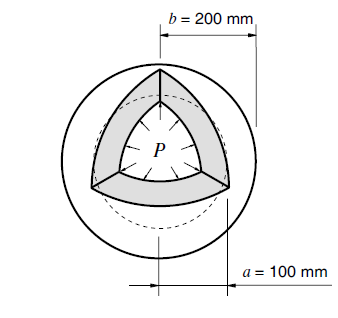
\includegraphics[width=200pt]{illustration_hollow_sphere.png}
\end{figure}

The material parameter follows:
\begin{figure}[!ht]
\center
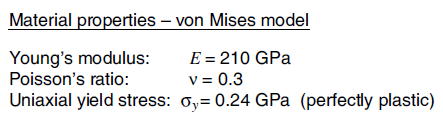
\includegraphics[width=200pt]{material_parameter.png}
\end{figure}

plastic yielding starts at the inner surface and
propagates through the shell as the internal pressure is increased. Collapse takes place when
the (spherical) plastic front reaches the outer boundary and the entire shell is under plastic
flow.

\section{Analytical Solution}
Consider a hollow sphere exerted by uniformly distributed pressure on inner surface, with magnitude $p$. The internal and external radii of the sphere is denoted by $a$ and $b$ respectively.
In pure elastic case, the Lame solution gives the stress components in spherical polar coordinates:
\begin{align}
\sigma_r=&-p\frac{\frac{b^3}{r^3}-1}{\frac{b^3}{a^3}-1}\\
\sigma_{t}=&p\frac{\frac{b^3}{2r^3}+1}{\frac{b^3}{a^3}-1}
\end{align}
where $\sigma_r$ is the radial stress and $\sigma_t$ is the hoop stress.The displacement is:
\begin{equation}\label{eq:displacement_elastic}
u=\frac{p}{E}\frac{(1-2\mu)r+\frac{(1+\mu)b^3}{2r^2}}{\frac{b^3}{a^3}-1}
\end{equation}
With increasing pressure $p$ the sphere yields and plastic region propogates from inner sphere to outer region. The elastic region($c\leq r \leq b$) can still be regarded as a "sphere":
\begin{align}
\sigma_r=&-A(\frac{b^3}{r^3}-1)\\
\sigma_{t}=&A(\frac{b^3}{2r^3}+1)
\end{align}
The sphere surface $r=c$ is the boundary between plastic and elastic region, and the point on this boundary is on the yielding surface ($\sigma_t-\sigma_r=\sigma_y$)also.
Therefore,
\[
A=\frac{2c^3\sigma_y}{3b^3}
\]
The stress tensor is continuous across this boundary (but not differential),therefore we get the pressure at $r=c$:
\[
p_{c}=\frac{2c^3\sigma_y}{3b^3}(\frac{b^3}{c^3}-1)
\]
Replacing $a$ with $c$ and $p$ with $p_c$ in equation (\ref{eq:displacement_elastic}) we get the displacement in elastic region:
\begin{equation}
u=\frac{2\sigma_y c^3}{3Eb^3}\left((1-2\mu)r+\frac{(1+\mu)b^3}{2r^2}\right),c\leq r\leq b
\end{equation}
In the plastic region $a\leq r\leq c$, from the equilibrium equation:
\[
\frac{\partial \sigma_r}{\partial{r}}=\frac{2(\sigma_t-\sigma_r)}{r}
\]
We get:
\begin{align}
\sigma_r=&-2\sigma_y\ln(\frac{c}{r})-\frac{2\sigma_y}{3}(1-\frac{c^3}{b^3})\\
\sigma_t=&\sigma_y-2\sigma_y\ln(\frac{c}{r})-\frac{2\sigma_y}{3}(1-\frac{c^3}{b^3})
\end{align}
From the boundary condtion at $r=a$, we can determine $c$ implicitly:
\begin{equation}
2\sigma_y\ln(\frac{c}{a})+\frac{2\sigma_y}{3}(1-\frac{c^3}{b^3})=p
\end{equation}
Below we determine the displacement $u(r)$ from the geometric equation:
\begin{align}
\epsilon_r=&\frac{\partial u}{\partial r}\\
\epsilon_t=&\frac{u}{r}
\end{align}
and constitutive equation between $(\sigma_r,\sigma_t)$ and $(\epsilon_r,\epsilon_t)$
We use the perfectly plastic model:$E_p=0$ and $\sigma_y=\sigma_t-\sigma_r$ is a constant.
By some calculation we get:
\begin{equation}
\binom{d\sigma_r}{d\sigma_t}=\left(\begin{matrix}
\lambda+\frac{2G}{3}&2\lambda+\frac{4G}{3}\\
\lambda+\frac{2G}{3}&2\lambda+\frac{4G}{3}
\end{matrix}\right)
\binom{d\epsilon_r}{d\epsilon_t}
\end{equation}
The matrix is singular, which is plausible since $d\sigma_r=d\sigma_t$.
Combiming with geometric equation we get the ODE for $u(r)$:
\begin{equation}
(\lambda+\frac{2G}{3})(r^2 u''(r)+2ru'(r)-2u(r))=2\sigma_y r
\end{equation}
Let $r=e^t$ and we can get the general solution for this equation:
\[
u(r)=\frac{c_1}{r^2}+(c_2+\frac{2\sigma_y \ln(r)}{3k})r,a\leq r \leq c
\]
where $k=\lambda+\frac{2G}{3}$,$c_1,c_2$ should be determined by the $C^1$ continuous of $u(r)$ at $r=c$.
\begin{align}
c_1=&\frac{c^3\sigma_y(5-\mu)}{3E}\\
c_2=&\frac{2\sigma_y(-1+2\mu)(b^3-3c^3+3b^3\ln(c))}{3b^3E}
\end{align}
\newpage
\section{FEM result}
\begin{figure}[!ht]
\center
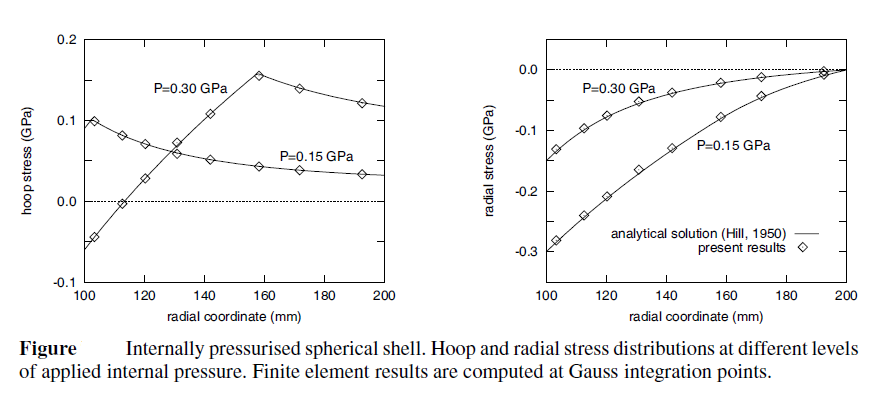
\includegraphics[width=300pt]{hollow_sphere_fem_result.png}
\end{figure}
\section{Numerical Solution}
We use incremental FEM method to solve this elasto-plastic problem.
\begin{thebibliography}{9}
\bibitem{NO}
  \textit{COMPUTATIONAL METHODS FOR PLASTICITY:THEORY AND APPLICATIONS} 7.5.2
\end{thebibliography}


\end{document}
